% !TeX root = ../main.tex
% Add the above to each chapter to make compiling the PDF easier in some editors.

\chapter{Comparison}\label{chapter:04_comparison}

In this section we are going to analyse the results of the first 15 testcases we got from the SteinerLib. We are going to constrast the solutions from the respective approximation with the optimal solution cost, which is referenced in the testcase database \cite{Dui93}. We are also going to look at the solution tree of testcase 41, its solution for the three algorithms differs substantially enough to nicely showcase their different approaches. The trees were output as a .dot file and visualized using the open source software "graphviz". 

\section{MST approximation}

In the table \ref{tab:MSTResults} we can see the results of MST approximation for the 15 testcases, that we are going to compare between the different algorithm. While these results all within close proximity to the optimal solution, with the biggest difference being the 441 difference for testcase 45. Overall the average performance for MST is quite good, but the problem with it is the bad worst case performance. Since MST only looks at the shortest paths between pairs of nodes it doesn't consider adding Steiner nodes, that have a largely reduced shortest cost to multiple terminals, if they don't appear in a shortest path directly. It is therefore largely dependant on the input graph and whilst it produces mostly good results it doesn't pick up on some potential cost reducing Steiner nodes, what the other algorithms improve on. We see this reflected in the output tree \ref{fig:MSTTree41}, that consists of direct connections between terminals and just one Steiner node, which is in the shortest path between the two respective nodes. 
\begin{table}[htbp]
 \caption{Results of MST for 15 testcases from SteinerLib \cite{Dui93}}\label{tab:MSTResults} 	
 \centering
 \begin{tabular}{l l l l}
\toprule
Graph & Opt & MST & MST-Opt \\
\midrule
11	& 1479	& 1585		& 106 \\
12	& 1484	& 1788		& 304 \\
13	& 1381	& 1676		& 295 \\
14	& 1397	& 1679		& 280 \\
15	& 1495	& 1602		& 107 \\
\midrule 
21	& 1175	& 1471		& 296 \\
22	& 1178	& 1477		& 299 \\
23	& 1174	& 1471		& 297 \\
24	& 1161	& 1473	 	& 312 \\
25	& 1162	& 1483		& 321 \\
\midrule
41	& 1276	& 1600		& 324 \\
42	& 1287	& 1674		& 387 \\
43	& 1295	& 1689		& 394 \\
44	& 1366	& 1676		& 310 \\
45	& 1310	& 1751		& 441 \\
\bottomrule
\end{tabular}
\end{table}

\begin{figure}[htbp]
\centering
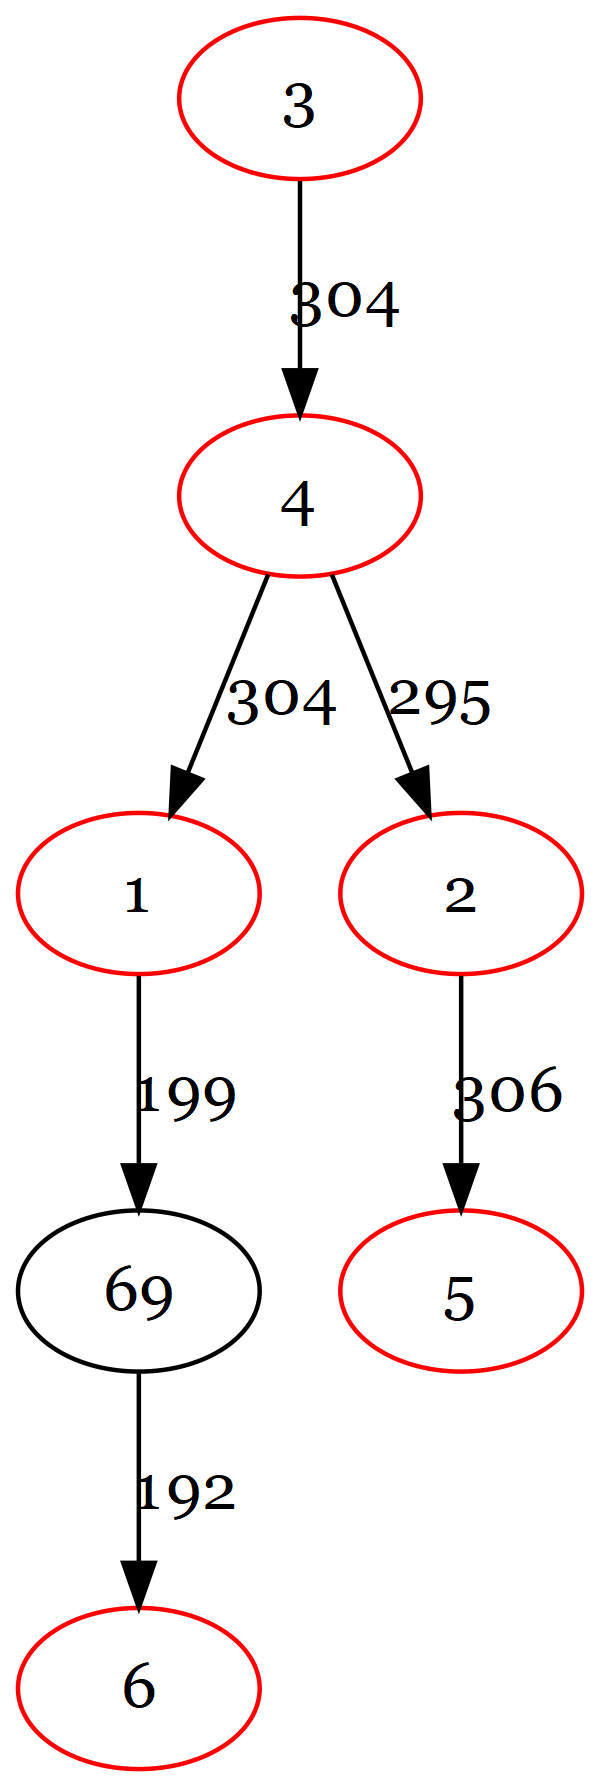
\includegraphics[scale=0.15]{figures/MST.png}
\caption{Output tree of the MST-approximation algorithm for Graph 41}\label{fig:MSTTree41}
\end{figure}

\section{Berman and Ramaiyer}

If we look at the results for the Berman, Ramaiyer algorithm (ref. \ref{tab:BeRaResults}) and contrast them with the MST results (ref. \ref{tab:MSTResults}) we can see that a lot of solutions have the same total treecost. This is to be expected because the Berman, Ramaiyer algorithm uses a MST-approximation as its input, which it tries to improve. So everytime it's unable to find such an improvement its output tree is identical to MST. Since Berman, Ramaiyer looks at subsets of terminals and checks whether the solution tree of that subset and the subsequent removal of redundant edges would lower the cost directly, its treecost is always lower than MST. It is also more dependable when it comes to the worst case performance with a PR of 1.734, but it still misses out on Steiner nodes that efficiently connect other Steiner nodes. When we look at the output tree \ref{BeRaTree41} we can see that it has included an additional Steiner node that connects 3 terminals and reduces the total tree cost by 22.
\begin{table}[htbp]
 \caption{Results of Berman, Ramaiyer for 15 testcases from SteinerLib \cite{Dui93}}\label{tab:BeRaResults} 	
 \centering
 \begin{tabular}{l l l l l}
\toprule
Graph & Opt & BeRa & BeRa\% & BeRa-Opt \\
\midrule
11	& 1479	& 1585	& 1.072	& 106 \\
12	& 1484	& 1788	& 1.205	& 304 \\
13	& 1381	& 1676	& 1.214	& 295 \\
14	& 1397	& 1679	& 1.202	& 282 \\
15	& 1495	& 1602	& 1.072	& 107 \\
\midrule 
21	& 1175	& 1471	& 1.252	& 296 \\
22	& 1178	& 1477	& 1.254	& 299 \\
23	& 1174	& 1471	& 1.253	& 297 \\
24	& 1161	& 1473	& 1.269 	& 312 \\
25	& 1162	& 1483	& 1.276	& 321 \\
\midrule
41	& 1276	& 1578	& 1.234	& 302 \\
42	& 1287	& 1658	& 1.288	& 371 \\
43	& 1295	& 1689	& 1.304	& 394 \\
44	& 1366	& 1676	& 1.227	& 310 \\
45	& 1310	& 1751	& 1.337	& 441 \\
\bottomrule
\end{tabular}
\end{table}

\begin{figure}[htbp]
\centering
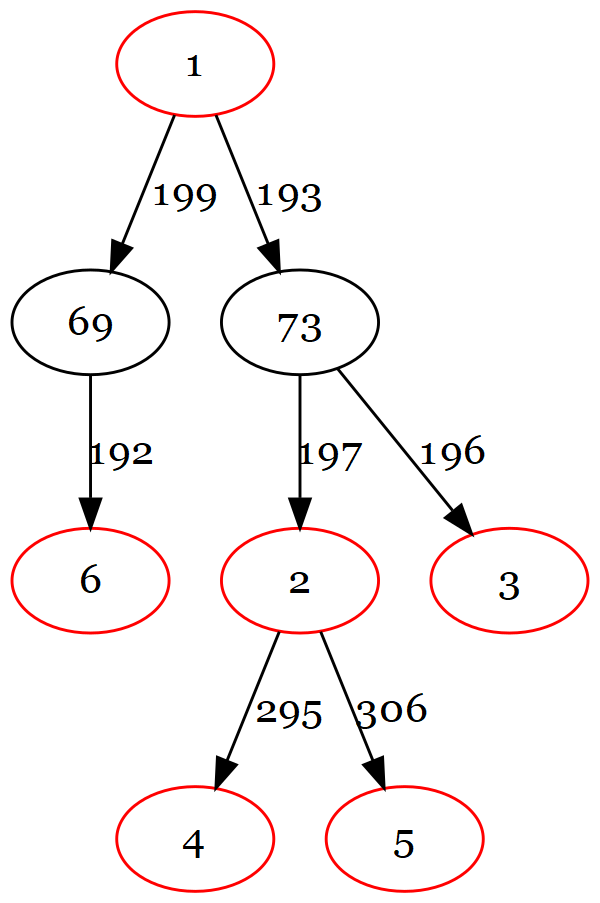
\includegraphics[scale=0.25]{figures/BermanRamaiyer.png}
\caption{Output tree of the Berman, Ramaiyer algorithm for Graph 41}\label{fig:BeRaTree41}
\end{figure}

\section{Hougardy and Proemel}

The results of Hougardy and Proemel's $IRGH$-algorithm (ref. \ref{tab:HoPrResults}) we can see that the treecosts aren't strictly better than the MST-approximation. This is due to the fact, that IRGH uses a heuristic that allows even the inclusion of subtrees, that have a negative effect on the tree cost to create more opportunities in the next iteration. This leads to its results being either significantly better than Berman,Ramaiyer or even worse than MST. Its performance ratio is also the best out of the three, since it is less likely to miss good Steiner nodes to include, because upon every addition of Steiner nodes it commences to check for additional Steiner nodes to connect the recently added ones. This strong incentive to include Steiner nodes is also visible in the output tree of testcase 41 (ref. \ref{fig:HoPrTree41}). It also shows, that $IRGH$ doesn't stick close to the solution of the initial MST-approximation like Berman, Ramaiyer does. There isn't a single edge belonging to the initial MST-approximation left in the output tree of $IRGH$.

\begin{table}[htbp]
 \caption{Results of $IRGH$ for 15 testcases from SteinerLib \cite{Dui93}}\label{tab:HoPrResults} 	
 \centering
 \begin{tabular}{l l l l l}
\toprule
Graph & Opt & HoPr & HoPr\% & HoPr-Opt \\
\midrule
11	& 1479	& 1654	& 1.118	& 175 \\
12	& 1484	& 1759	& 1.185	& 275 \\
13	& 1381	& 1471	& 1.065	& 90 	\\
14	& 1397	& 1848	& 1.323	& 451 \\
15	& 1495	& 1895	& 1.268	& 400 \\
\midrule 
21	& 1175	& 1471	& 1.252	& 296 \\
22	& 1178	& 1477	& 1.254	& 299 \\
23	& 1174	& 1471	& 1.253	& 297 \\
24	& 1161	& 1473	& 1.269 	& 312 \\
25	& 1162	& 1483	& 1.276	& 321 \\
\midrule
41	& 1276	& 1463	& 1.147	& 187 \\
42	& 1287	& 1631	& 1.267	& 344 \\
43	& 1295	& 1535	& 1.185	& 240 \\
44	& 1366	& 1546	& 1.132	& 180 \\
45	& 1310	& 1616	& 1.234	& 306 \\
\bottomrule
\end{tabular}
\end{table}

\begin{figure}[htbp]
\centering
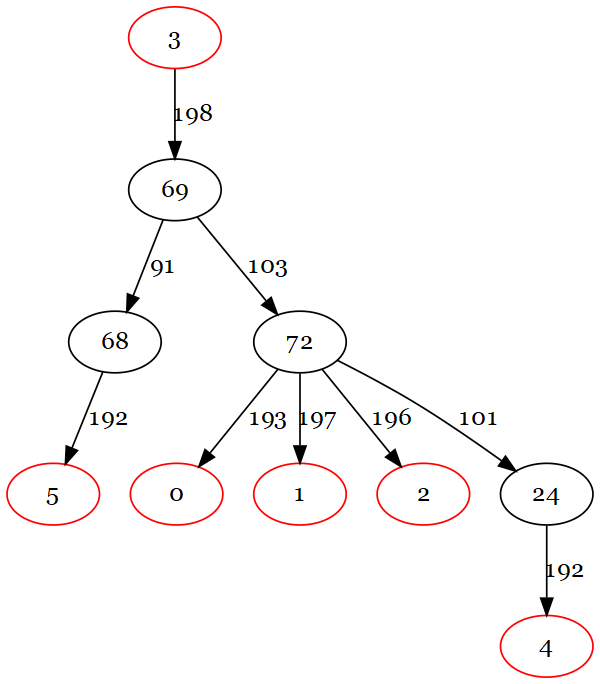
\includegraphics[scale=0.40]{figures/HougardyProemel.png}
\caption{Output tree of the $IRGH$-approximation algorithm for Graph 41}\label{fig:HoPrTree41}
\end{figure}
